\chapter{مقدمه}
\subsection{مقدمه ای بر \lr{5G} }
\lr{5G}،
مخابرات نسل پنجم
سیستم های بیسیم \LTRfootnote{Wireless} وشبکه های مخابراتی بعد از نسل چهارم می باشد که تکاملی از لایه ی فیزیکی در تکنولوژی شبکه های مخابراتی سیار همانند \lr{LTE} می باشد که نسبت به \lr{4G} سرعت و پوشش بهتری را فراهم می کند.  
\lr{5G}
نوع جدیدی از شبکه را ایجاد می کند که به منظور اتصال تقریبا همه و همه چیز با هم از جمله ماشین ها، اشیاء و دستگاه ها ساخته شده است.
\lr{5G}
 فناوری بی سیم برای ارائه سرعت داده های چند گیگابیت بر ثانیه ، تأخیر فوق العاده کم ، قابلیت اطمینان بیشتر ، ظرفیت شبکه گسترده، افزایش در دسترس بودن و تجربه کاربری یکنواخت تر به کاربران بیشتر است. عملکرد بالاتر و بهره وری بهبود یافته باعث افزایش تجربیات کاربر جدید شده و صنایع جدیدی را به هم متصل می کند.
 
 
تکنولوژی سیگنال  \lr{5G} برای پوشش فراگیرتر و بازدهی بهتر سیگنال ایجاد شده است. این پیشرفت ها منجر به تغییراتی از قبیل\lr{IOT} \LTRfootnote{Internet of Things} و \lr{Pervasive Computing} در آینده ی نزدیک خواهد شد.
همچنین \lr{5G} منجر به توسعه و بهبود سرویس های مخابراتی و اینترنتی سیار و در ورای آن، ایجاد تجربه ی بهتری برای مصرف کنندگان خواهد شد.\newline
برای توسعه ی اینترنت سیار و \lr{IOT}، نیاز داریم تا شبکه های\lr{5G}، معنای اولیه برای دسترسی شبکه برای ارتباط انسان ها با یکدیگر و ارتباط ماشین با انسان گردد.
به طور کلی، 
\lr{5G}
 در سه نوع سرویس اصلی متصل از جمله پهن باند تلفن همراه، IoT عظیم و ارتباطات مهم برای ماموریت استفاده می شود.
\begin{enumerate}
\item 
پهن باند تلفن همراه پیشرفته 
\lr{(eMBB)}
 برای مقابله با نرخ داده های بسیار زیاد ، تراکم بالای کاربران و ظرفیت ترافیک بسیار بالا برای سناریوهای مختلف و همچنین پوشش یکپارچه و سناریوهای تحرک بالا با نرخ داده های استفاده شده بهبود یافته است.
\item
 ارتباطات  عظیم ماشین 
 \lr{(mMTC)}
  برای
\lr{IoT}،
   برای تعداد بسیار زیاد دستگاههای متصل به مصرف کم و نرخ داده کم نیاز دارد.
\item 
ارتباطات بسیار مطمئن و با تأخیر کم
 \lr{(URLLC)}
 برای برنامه های کاربردی مهم برای ایمنی و ماموریت
  مهم است.
\end{enumerate}
 از آنجا که
\lr{5G}
 تکامل می یابد و کمتر به زیرساخت های \lr{4G} وابسته می شود و طیف بیشتری در دسترس قرار می گیرد،
 تخمین ها سرعت بارگیری را حداکثر 1000 برابر سریعتر از \lr{4G} قرار می دهد، که بالقوه از 
 \lr{10Gbps} 
بیشتر است، که به شما امکان می دهد تا در کمتر از یک ثانیه فیلم کامل
\lr{HD}
   را بارگیری کنید.
   برخی تخمین ها محافظه کارانه تر هستند ، اما حتی محافظه کارانه ترین آن را چندین ده برابر سریعتر از \lr{4G} قرار می دهد.
دلایل نیاز به نسل پنجم اینترنت به طور خلاصه در ادامه بیان شده است \citep{etsi}.
\begin{itemize}
\item ترافیک داده های تلفن همراه به دلیل پخش ویدئو به سرعت رو به افزایش است.
\item با در اخیار داشتن چندین دستگاه به طور همزمان، هر کاربر تعداد فزاینده ای از اتصالات را در اختیار دارد.
\item اینترنت اشیاء به شبکه هایی نیاز دارد که میلیاردها دستگاه را اداره کنند.
\item با وجود تعداد فزاینده ای از دستگاه های ارتباطی و افزایش ترافیک داده ها ، هم دستگاه ها و هم شبکه ی  
آن
نیازمند افزایش بهره وری انرژی هستند.
\item 
 به دلیل تحت فشار قرار گرفتن اپراتورهای شبکه برای کاهش هزینه های عملیاتی و همچنین به دلیل اینکه کاربران به تعرفه های نرخ مسطح عادت می کنند و مایل نیستند مبلغ بیشتری بپردازند.
\item فناوری ارتباطات سیار می تواند موارد استفاده جدیدی را ایجاد کند (به عنوان مثال موارد تاخیر فوق العاده کم یا قابلیت اطمینان بالا) و برنامه های جدید برای صنعت که منجر به درآمد زایی بیشتر اپراتورها می گردد.
\end{itemize}
بنابراین عملکرد عملیاتی نسل پنجم می بایست به طور قابل توجهی افزایش یابد (به عنوان مثال افزایش راندمان طیفی ، سرعت بالاتر داده ، تأخیر کم).
\lr{5G}
می بایست
در حالی که هنوز سطح قابل قبولی از مصرف انرژی ، هزینه تجهیزات و استقرار شبکه و هزینه بهره برداری را ارائه می دهد،
 اینترنت اشیاء را به طور گسترده نیز تأمین کند.
 همچنین می بایست 
از طیف گسترده ای از برنامه ها و خدمات پشتیبانی کند.
 \begin{figure}[H]
  \centering
    \includegraphics[width=0.8\textwidth]{./fig/etsi}
  \caption{مقایسه قابلیت های کلیدی
\lr{IMT-Advanced}
 (نسل 4) با
\lr{IMT-2020}
 (نسل ۵) 
 با توجه به
\lr{ITU-R M.2083}
\cite{etsi}
  }
  \label{fig:C-RAN}
\end{figure}
\subsection{تاریخچه مخابرات}
در ابتدا می خواهیم بدانیم که چه چیزی منجر به رفتن محققان به سوی  \lr{5G} شده است. یکی از دلایل مهم، سرعت و نرخ انتقال بیشتری است که در ادامه به آن می پردازیم.
نیاز بشریت به ارتباط تلفنی (انتقال بدون سیم به صورت زمان حقیقی \LTRfootnote{Real Time} انسان را به سمت نسل اول ارتباطات \lr{1G} سوق داده است. نسل دوم ارتباطات \lr{2G} با سرویس های انتقال پیام کوتاه ایجاد شد. همچنین با موفقیت تکنولوژی شبکه های منطقه ای بیسیم، اتصال به داده های اینترنتی مورد توجه عموم مردم قرار گرفت که پلی به سوی نسل سوم ارتباطات \lr{3G} را فراهم نمود. به طور منطقی پله ی بعدی گام برداشتن در راستای کوچک شدن لپ تاپ و در آمیختن آن با تلفن که امروزه به صورت تلفن هوشمند\LTRfootnote{smart phone} است و دسترسی به  اینترنت، پهنای باند بالا و داده ها در نقاط مختلف جهان بوده است که \lr{4G} یا نسل چهارم را به همراه داشته است.
با توجه به افزایش تعداد کاربران تلفن های
هوشمند و تبلت ها و افزایش نرخ ارسال اطلاعات و داده ها در طی سال
های اخیر طبق پیش بینی های سیسکو میزان ترافیک \lr{IP} طی سالهای اخیر
  چندین برابر افزایش خواهد یافت.
در نتیجه اپراتورها برای حل این مشکل و خدمات
دهی بهتر ناچار به افزایش ظرفیت شبکه می باشند.
در ادامه به طور مختصر به ۵ نسل مخابراتی می پردازیم\cite{Gen}.
\subsubsection{نسل اول}
این اولین نسل از فناوری تلفن همراه بود. اولین نسل شبکه تلفن همراه تجاری در اواخر دهه 70 معرفی شد و استانداردهای کاملاً اجرا شده در دهه 80 تاسیس شد. استرالیا در سال 1987 توسط \lr{Telecom} (که امروزه با عنوان \lr{Telstra} شناخته می شود) معرفی شد ، استرالیا اولین شبکه تلفن همراه خود را با استفاده از یک سیستم آنالوگ \lr{1G} دریافت کرد. \lr{1G} یک فناوری آنالوگ است و به طور کلی تلفن ها از باتری ضعیف برخوردار هستند و کیفیت صدا بدون امنیت بسیار زیاد بود و گاهی اوقات تماس های کاهش یافته را تجربه می کنید. این استانداردهای ارتباطی آنالوگ ارتباطی است که در دهه 1980 معرفی شد و تا زمانی که جایگزین ارتباطات دیجیتال \lr{2G} شود ، ادامه یافت. حداکثر سرعت \lr{1G} 2.4 کیلوبیت بر ثانیه است.
\subsubsection{نسل دوم}
تلفنهای همراه وقتی از \lr{1G} به \lr{2G} رفتند ، اولین نسخه اصلی خود را دریافت کردند. تفاوت اصلی بین دو سیستم تلفن همراه (\lr{1G} و \lr{2G}) در این است که سیگنالهای رادیویی مورد استفاده شبکه \lr{1G} آنالوگ هستند ، در حالی که شبکه های 
\lr{2G}
 دیجیتال هستند. انگیزه اصلی این نسل، تهیه کانال ارتباطی ایمن و مطمئن بود. این نسل همچنین مفهوم \lr{CDMA} و \lr{GSM} را پیاده سازی کرد که خدماتی مانند پیامک را ارائه داده است. شبکه های مخابراتی سلولی نسل دوم بطور تجاری در سال 1991 توسط رادیولینجا (در حال حاضر بخشی از الیزا اویج) توسط استاندارد \lr{GSM} در فنلاند راه اندازی شد.
\lr{2G}
قابلیت هایی از قبیل
\lr{multiplexing}
دارد که 
به چندین کاربر در یک کانال منفرد 
اجازه ی انتقال داده می دهد.
انتقال داده و صدا در این نسل وجود داشته است.
در این نسل مخابرات، 
سرویسهای اساسی مانند پیام کوتاه، رومینگ داخلی، تماس های کنفرانسی، نگه داشتن تماس و صورتحساب مبتنی بر خدمات معرفی شده است. جداسازی هزینه های مبتنی بر تماس های مسافت طولانی و صورتحساب در زمان واقعی نیز از قابلیت های این نسل بود.
حداکثر سرعت برای سرویس \lr{GPRS}
\LTRfootnote{General Packet Radio Service}
\lr{50Kbps}
و برای سرویس 
\lr{EDGE}
\LTRfootnote{Enhanced Data Rates for GSM Evolution}
\lr{1Mbps}
می باشد.
\subsubsection{نسل سوم}
این نسل مخابراتی استانداردهای بسیاری از فناوری های بیسیم را تعیین نمود. مرورگر وب ، ایمیل ، بارگیری ویدیو ، به اشتراک گذاری عکس و سایر فناوری های هوشمند در نسل سوم معرفی شدند که در سال 2001 به طور تجاری معرفی شد. اهداف تعیین شده برای ارتباطات سیار نسل سوم، تسهیل ظرفیت بیشتر صدا و داده ، پشتیبانی از طیف گسترده تری از برنامه ها و افزایش انتقال داده با هزینه کمتری بود.
استاندارد \lr{3G} از فناوری جدیدی به نام
 \lr{UMTS}
 \LTRfootnote{Universal Telecommunications System Mobile}
 به عنوان معماری اصلی شبکه خود 
استفاده می کند.
\lr{3G}
 دارای پشتیبانی خدمات چندرسانه ای است.
\lr{3G}
  با بهبود چگونگی فشرده سازی صدا در طی تماس، راندمان طیف فرکانس را افزایش داده است، بنابراین تماس همزمان بیشتری می تواند در همان محدوده فرکانس اتفاق بیفتد.
حداکثر سرعت این نسل 
\lr{2Mbps}
و
حداکثر سرعت نظری برای HSPA + 21.6 Mbps است. 
\subsubsection{نسل چهارم}
\lr{4G}
 یک فناوری بسیار متفاوت در مقایسه با \lr{3G} است و هدف از آن ، فراهم آوردن سرعت بالا ، کیفیت بالا و ظرفیت بالا برای کاربران در عین بهبود امنیت و کاهش هزینه خدمات صوتی و دیتا ، چندرسانه ای و اینترنت از طریق \lr{IP} می باشد. برنامه های کاربردی بالقوه و جاری شامل دسترسی به وب موبایل اصلاح شده ، تلفن تلفنی \lr{IP}، خدمات بازی، تلویزیون همراه با کیفیت بالا ، کنفرانس ویدیویی، تلویزیون سه بعدی و محاسبات ابری از قابلیت های پشتیبانی آن می باشد.

فن آوری های کلیدی که این امکان را ایجاد کرده اند 
\lr{MIMO} \LTRfootnote{Multiple Output Multiple Output}
 و
  \lr{OFDM} \LTRfootnote{Multiplexing Division Frequency Division}
می باشد.
دو استاندارد مهم آن
\lr{LTE} \LTRfootnote{Long Term Evolution}
و
\lr{WiMAX}
می باشد.
حداکثر سرعت یک شبکه 4G هنگام حرکت دستگاه 100 مگابیت بر ثانیه یا 1 گیگابیت بر ثانیه برای ارتباطات کم تحرک مانند هنگام ایستادن یا راه رفتن است. تأخیر از حدود \lr{300ms} به  \lr{100ms} با کاهش تراکم دست می یابد.
 \subsubsection{نسل پنجم}
 با توجه
به این که نرخ داده و ظرفیت در سیستم های نسل چهارم به ظرفیت
شانون نزدیک شده است، در نتیجه روش هایی که برای
افزایش ظرفیت شبکه مورد استفاده می گیرند که به شرح زیر است:
\begin{itemize}
\item
استفاده از تکنیک \lr{Massive Mimo}
\item
استفاده از روش های پردازش های ابری
\item
شبکه ی تعریف شده ی نرم افزاری
\lr{SDN}
\LTRfootnote{Software Defined Networking}
\item
موج میلیمتری
\LTRfootnote{mm Wave}
\item 
ساختار شبکه های دسترسی رادیویی باز
\lr{ORAN}
\LTRfootnote{Open Radio Access Network}
\item 
مجازی سازی توابع شبکه
\lr{NFV}
\LTRfootnote{Network Function Virtualization}
\item 
برش شبکه
\LTRfootnote{Network Slicing}
\end{itemize}
\section{مقدمه ای بر ساختار \lr{ORAN}}
مجازی سازی \lr{RAN} توجه زیادی را از طرف اپراتورها به خود جلب می کند ، زیرا منجر به کاهش هزینه های اپراتور و \lr{opex} می شود و همچنین این امکان را برای آنها فراهم کند تا با سرعت بیشتری قابلیت های جدیدی به شبکه اضافه کنند.

این احتمال وجود دارد که همه این علاقه ها در ایجاد سه گروه مختلف باشد -
 انجمن 
 \lr{xRAN} 
 ، گروه
 \lr{ OpenRAN }
  شرکت 
 \lr{ Telecom Infra}
   و ابتکار عمل
\lr{Open VRAN}
که برای شرکت سیسکو می باشد.
اگرچه همه این گروه ها می گویند که در حال کار بر روی یک چیز هستند، که اساساً برای باز کردن \lr{RAN} با استفاده از رابط های استاندارد و عناصر شبکه جعبه سفید است، اما در بررسی دقیق تر اختلافاتی نیز وجود دارد.

\lr{Open RAN}(\lr{ORAN})
تبسیط و ترکیبی از دو ساختار \lr{C-RAN} \LTRfootnote{Cloud Radio Access Network} و \lr{xRAN} می باشد که انتظار می رود که در فناوری نسل پنجم مخابرات مورد استفاده قرار گرفته و منجر به بهبود عملکرد شبکه های دسترسی رادیویی \lr{RAN} گردد. 
این ساختار یک شبکه ی باز، انعطاف پذیر و هوشمند است.


\lr{ORAN} 
توابع
 شبکه ی دسترسی رادیویی 
 را به سه قسمت تقسیم می کند،
  که قسمت اول واحد از راه دور
 \lr{(RU)} \LTRfootnote{remote unit} 
 ، واحد توزیع شده
  \lr{(DU)} \LTRfootnote{Distributed unit} 
  و واحد مرکزی 
   \lr{(CU)} \LTRfootnote{Central unit} 
   می باشد.
   در حالی که  \lr{RU} دارای توابع  \lr{(PHY)} \LTRfootnote{Physical layer} پایین تر است،
    \lr{DU} حاوی \lr{(PHY)} بالاتر، 
    \lr{MAC} 
 \LTRfootnote{Medium Access Control}   
    و
     \lr{RLC}
   \LTRfootnote{Radio Link Control}  
      است     
    و 
    \lr{(CU)}
     حاوی
     \lr{RRC}
     \LTRfootnote{Radio Resource Control}
      ،\lr{PDCP}
      \LTRfootnote{Packet Data Convergence Protocol}
      و 
      \lr{SDAP}
      \LTRfootnote{Service Data Adaptation Protocol}
      است.
      
\lr{DU}
و
\lr{CU}
به عنوان توابع شبکه مجازی \lr{(VNFs)} پیاده سازی می شوند،
که در یک محیط ابر اجرا می شود.

رابط های بین \lr{RU} ، \lr{CU} و \lr{DU} رابط های استاندارد باز هستند.
\subsection{مقدمه ای بر \lr{C-RAN}}
شبکه های دسترسی ابری منجر به افزایش پوشش ارسالی می گردد. با توجه به ساختار شبکه
   \lr{C-RAN} که معماری جدیدی را برای شبکه های نسل آینده
ارائه می دهد، نه تنها ظرفیت شبکه افزایش می یابد بلکه
مشکلاتی که در روش های دیگر وجود دارد را نیز هموار
می سازد.
مفهوم شبکه دسترسی رادیو ابر \lr{C-RAN}، به مجازی سازی کارکردهای ایستگاه  پایه \LTRfootnote{Base Station-BS} با استفاده از تکنولوژی رایانش ابری \LTRfootnote{Cloud Computing} اشاره می نماید. این مفهوم به ایجاد یک ساختار سلولی جدید منجر می شود که در آن، نقاط دسترسی بیسیم کم هزینه که با عنوان واحدهای رادیویی \LTRfootnote{Radio Units} و یا رادیو هد های
  راه دور 
  \LTRfootnote{Radio Remote Heads}
 شناخته می شوند- با استفاده از یک ابر متمرکز با قابلیت پیکربندی مجدد و یا واحد مرکزی \LTRfootnote{Control Unit} مدیریت می شوند. شبکه امکان کاهش هزینه های سرمایه گذاری و عملیاتی مورد نیاز برای اپراتور ها به منظور توسعه و نگهداری شبکه های ناهمگن متراکم را فراهم می آورد. این مزیت مهم در کنار بازده طیفی، تسهیم آماری \LTRfootnote{Statisitical Multiplexing}، و مزیت های متعادل سازی بار باعث می شود تا شبکه \lr{C-RAN} به عنوان یکی از تکنولوژی های کلیدی در توسعه سیستم های \lr{5G} در جایگاه بسیار مناسبی قرار بگیرد. در ادامه، یک بررسی کلی و مختصر از تحقیقات جدید در مورد ساختار \lr{C-RAN} ارائه می شود و موضوعات مورد تاکید عبارتند از فشرده سازی لینک \lr{fronthaul} پردازش باند پایه، کنترل دسترسی به محیط واسط، تخصیص منابع، ملاحظات سطح سیستم، و تلاش های انجام شده در راستای ارائه استاندارد ها.
\subsubsection{ساختار شبکه های مختلف }
با توجه به مقاله ی\cite{checko2015cloud}،
\begin{figure}
  \centering
    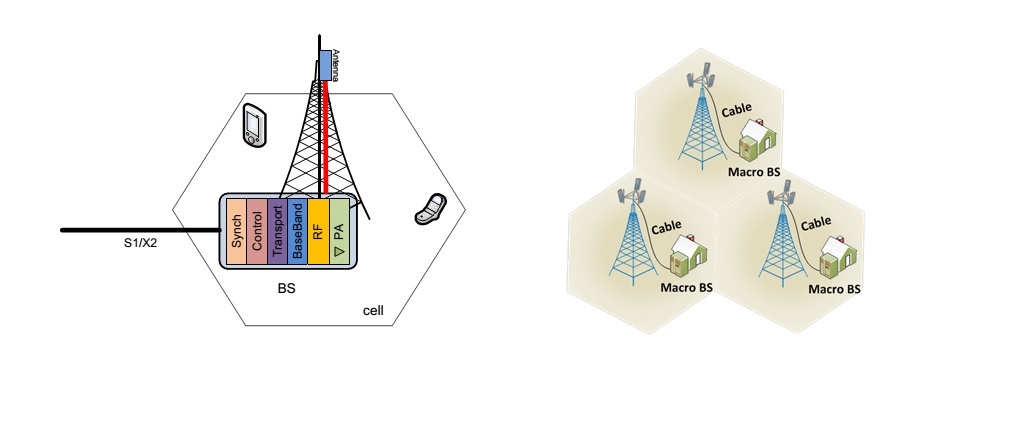
\includegraphics[scale=0.7]{./fig/c11}
  \caption{ساختار سنتی ایستگاه پایه \cite{checko2015cloud}}
  \label{fig:c11}
\end{figure}
هر ایستگاه پایه دو نوع پردازش انجام می دهد : پردازش
رادیویی که توسط واحد رادیویی \LTRfootnote{RRH} انجام می شود و شامل پردازش
دیجیتالی، فیلترینگ فرکانسی، تقویت توان و ....میباشد و
پردازش باند پایه که توسط واحد باند پایه \LTRfootnote{BBU} که همان واحد کنترل است \LTRfootnote{CU} انجام شده و از جمله
مهمترین وظایف آن می توان به کدینگ، مدولاسیون و
تبدیل فوریه ی سریع اشاره کرد. در ساختار جدیدی که
تحت عنوان \lr{C-RAN}  معرفی خواهیم نمود نحوه ی ارتباط
پردازشگرهای رادیویی و باند پایه متحول شده و در نتیجه
مزایایی برای شبکه حاصل خواهد شد.در ادامه ، انواع ساختارها را بیان خواهد شد.
\subsubsection{ساختار سنتی ایستگاه پایه }

در ساختارهای سنتی ایستگاه پایه، پردازش های رادیویی و باند پایه در
داخل ایستگاه پایه انجام می شد و مدول آنتن نیز در فاصله
ی چند متری از مدول رادیویی نصب شده و ارتباط آنها
توسط کابل کواکسیال برقرار می شد که همین امر سبب
افزایش تلفات در شبکه می باشد. این نوع ساختار در شکل
\ref{fig:c11} نشان داده شده است. همان گونه که مشاهده می کنید
ارتباط بین ایستگاههای پایه توسط ارتباط  $X_2$ و ارتباط بین
ایستگاه پایه و شبکه ی هسته توسط ارتباط $ S_1$ برقرار می
شود. این نوع ساختار در شبکه های \lr{1G} و \lr{2G} به کار گرفته
شده است 
\cite{checko2015cloud}.

%Figure \ref{fig:gull} shows a photograph of a gull.
\subsubsection{ ساختار ایستگاه پایه و واحد رادیویی}

\begin{figure}
  \centering
    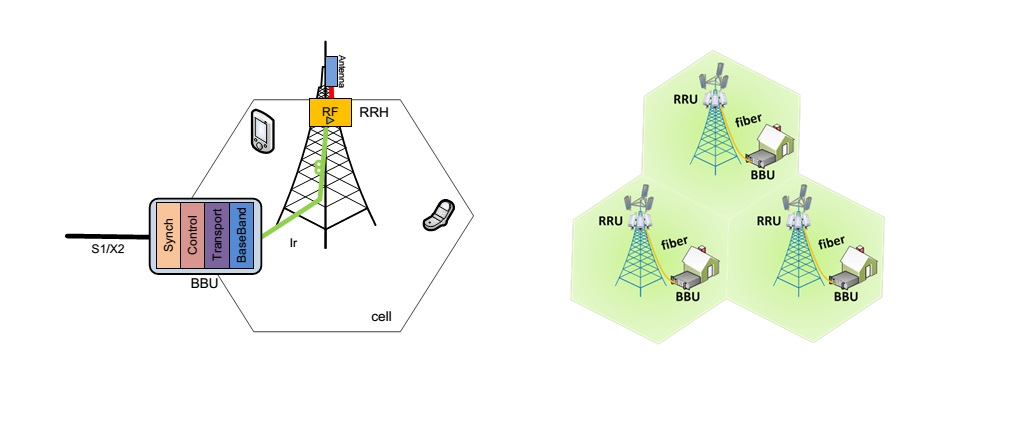
\includegraphics[scale=0.7]{./fig/c22}
  \caption{ ساختار ایستگاه پایه و واحد رادیویی \cite{checko2015cloud}}
  \label{fig:c22}
\end{figure}
در این ساختار واحد رادیویی و واحد پردازشی سیگنال، از هم
مجزا شده و واحد رادیویی که تحت عنوان \lr{RRH} یا \lr{RRU}
نیز شناخته می شود، توسط فیبر نوری به واحد باند پایه یا \lr{BBU} اتصال می
یابد. همان طور که پیشتر بیان شد واحد رادیویی مسئولیت
انجام پردازش های دیجیتالی از جمله تبدیل انالوگ به
دیجیتال، دیجیتال به انالوگ، تقویت توان و فیلترینگ رابر عهده دارد، که تفکیک وظایف واحد پردازشی و واحد
رادیویی در این ساختار در شکل \ref{fig:c22} قابل مشاهده است. این
نوع ساختار برای شبکه های نسل سوم معرفی شده و امروزه
نیز بیشتر ایستگاههای پایه از همین ساختار بهره می گیرند.
از جمله ویژگی های بارز این ساختار امکان ایجاد فاصله
بین واحد رادیویی و پردازشی می باشد، که این فاصله به
دلیل تاخیر پردازشی و انتشاری نمی تواند از  $40$کیلومتر
فراتر رود. در این ساختار تجهیزات مرتبط با \lr{BBU} می
توانند به مکانی مناسبتر که قابل دسترس تر بوده و هزینه
ی اجاره و نگهداری کمتری را به اپراتورها تحمیل می
کنند منتقل شوند و واحد های رادیویی نیز در در پشت بام
ساختمان ها و مکان های مرتفع نصب می شوند که این
خود سبب کاهش هزینه های خنک سازی ادوات موجود
می شود. نحوه ی ارتباط بین \lr{RRH} و \lr{BBU} مشابه ساختار
سنتی بوده و \lr{RRH} ها نیز توسط معماری زنجیروار با هم
در ارتباطند.
\begin{figure}[H]
  \centering
    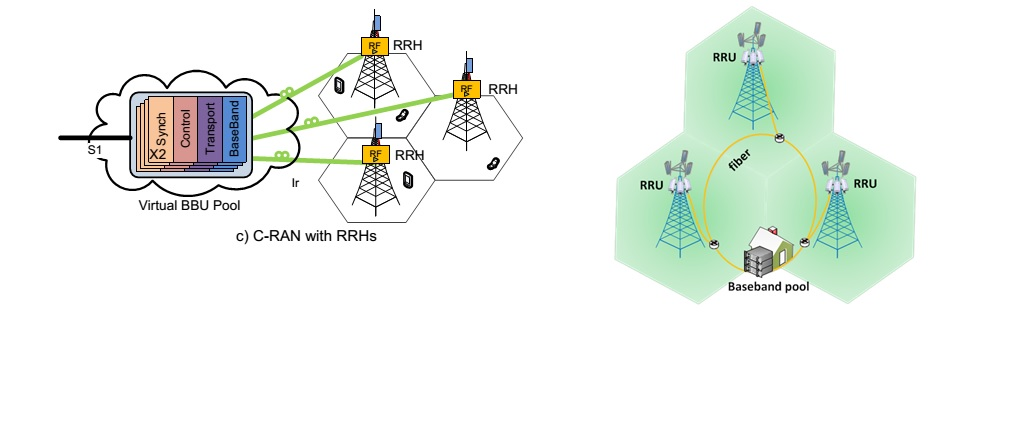
\includegraphics[scale=0.7]{./fig/c33}
  \caption{ساختار  \lr{C-RAN} \cite{checko2015cloud}}
  \label{fig:c33}
\end{figure}
\subsubsection{ساختار \lr{C-RAN}}




ایده اصلی \lr{C-RAN} جداسازی بخش رادیویی (\lr{RRH}) 
\LTRfootnote{Radio Remote Head}
 از واحد پردازشی باند پایه (\lr{BBU})
 \LTRfootnote{Baseband Unit}
  است.
از تجمیع \lr{BBU} ها بر روی سرور ابری، \lr{BBU-Pool} ایجاد می شود.
در این ساختار، در راستای بهینه سازی عملکرد \lr{BBU}
 ها در مواجهه باایستگاههای پایه پر ترافیک و کم ترافیک،
 \lr{BBU}ها به صورت یک مجموعه ی واحد تحت عنوان 
\lr{BBU Pool}
 در آمده اند که این مجموعه بین چندین سلول 
 به اشتراک گزارده شده و مطابق شکل زیر مجازی سازی
می شود. 
در توضیح بیشتر این ساختار می توان این گونه
عنوان کرد که \lr{BBU Pool} به عنوان یک خوشه ی مجازی
در نظر گرفته می شود که شامل پردازش گرهایی می باشد
که پردازش های باند پایه را انجام می دهند. ارتباط بین
  \lr{BBU}ها در ساختار های فعلی به شکل  $X_2$ برقرار می شود
که در این ساختار ارتباط بین خوشه ها از فرم جدید $X_2$
تحت عنوان  $X_2 +$برقرار می شود.
\newline
در شکل \ref{fig:C-RAN} ساختار کلی شبکه ی  \lr{C-RAN} در سیستم های
\lr{ LTE}
 نمایش داده شده است. همان طور که در شکل قابل
مشاهده می باشد ساختار کلی شبکه  \lr{C-RAN} به دو بخش
 \lr{backhaul} و \lr{fronthaul} تقسیم بندی شده است. بخش
 \lr{fronthaul}شبکه به مرحله ی اتصال سایت های \lr{ RRH}به
 به \lr{BBU Pool} به اتصال \lr{backhaul} و بخش \lr{BBU Pool}
هسته ی شبکه ی سیار اطلاق می شود. همان گونه که قبلا
ذکر شد  \lr{ RRH}ها در نزدیکی انتن نصب شده و از طریق
لینک های انتقالی نوری با پهنای باند وسیع و تاخیر کم به
پردازشگرهای قوی در  \lr{BBU}متصل می شوند. توسط این
لینک های انتقالی است که سیگنال های دیجیتالی باند
پایه از نوع \lr{IQ} بین \lr{RRH} و \lr{BBU} انتقال می یابند \cite{checko2015cloud}.
\begin{figure}[H]
  \centering
    \includegraphics[width=\textwidth]{./fig/CRAN}
  \caption{ساختار شبکه ی \lr{C-RAN} \cite{checko2015cloud}}
  \label{fig:C-RAN}
\end{figure}
\subsection{\lr{xRAN}}
\lr{xRAN}
در سال ۲۰۱۶ با هدف استانداردسازی یک جایگزین انعطاف پذیر و باز برای \lr{RAN}
مبتنی بر سخت افزار سنتی بدست آمده است.
 در این ساختار، سه حوزه ی مهم مورد بررسی قرار گرفته است.
اولین حوزه ی مورد بررسی، جداسازی بخش
صفحه ی کنترل
 \LTRfootnote{control plane} از 
 صفحه ی کاربر
\LTRfootnote{user plane}
می باشد. حوزه ی دوم،
ساختن یک پشته نرم افزاری \lr{eNodeB} مدولار که از سخت افزار \lr{COTS} استفاده می کند، می باشد.
حوزه ی سوم مورد بررسی، انتشار رابط های باز شمال و جنوب است
\cite{xran}.
\begin{itemize}
\item \textbf{ جداسازی بخش صفحه ی کنترل از 
صفحه ی کاربر}:
این انتقال صفحه ی کنترل، که قبلاً کاملاً به دستگاههای سخت افزاری \lr{RAN} متصل بود، به دستگاههای محاسباتی در دسترس امکان می دهد \lr{RAN} بتواند به عنوان یک استخر منطقی از ظرفیت ، با کارایی بیشتری کار کند.
نرم افزار \lr{eNodeB} از سخت افزار خاص فروشنده جدا می شود و الهام بخش نوآوری در هر دو نرم افزار و سخت افزار به صورت مشارکتی اما به طور مستقل است.
برنامه نویسی و کنترل زمان واقعی بی سابقه در زیرساخت های \lr{RAN} به دست آمده است، که به راحتی از برنامه های کاربردی تلفن همراه و خدمات تجاری پشتیبانی می کند.
\item \textbf{ساختن یک پشته نرم افزاری \lr{eNodeB} مدولار}:
رویکرد \lr{xRAN} به خوبی با طرح های مجازی سازی عملکرد شبکه حامل \lr{(NFV)} مطابقت دارد، و همچنین منجر به کنترل عملکرد ترافیک با کارایی بالا، مدیریت تداخل و کنترل منابع رادیویی روی سیستم عامل های استاندارد \lr{x86} و می شود.
\item \textbf{انتشار رابط های باز شمال و جنوب}: 
رابط های استاندارد و باز قابیت پشتیبانی از فروشنده های متعدد همکاری اثبات شده دارند. 
\lr{xRAN.org}
و اعضای آن به تصویب رساندن این رابط ها از طریق فرآیندهای استاندارد منجر به در دسترس قرار دادن معماری \lr{xRAN} و پشتیبانی مورد نیاز می شوند.
\cite{xran1}
\end{itemize}
\subsection{\lr{ORAN}}
معماری \lr{ORAN} برای ایجاد زیرساخت های \lr{RAN} نسل بعدی طراحی شده است.
معماری \lr{ORAN} با تکیه بر اصول هوشمندی و باز بودن، پایه و اساس ساخت \lr{RAN} مجازی بر روی سخت افزار آزاد ، با کنترل رادیویی ایجاد شده توسط هوش مصنوعی است که توسط اپراتورهای سراسر جهان پیش بینی شده است.
این معماری بر روی رابط های استاندارد و تعریف شده ای بنا شده است تا یک زنجیره اکوسیستم با قابلیت باز ایجاد کند که دارای پشتیبانی کامل از استانداردهای تبلیغ شده توسط \lr{3GPP} و سایر سازمان های استاندارد صنعت فراهم شود.
\begin{figure}[H]
  \centering
    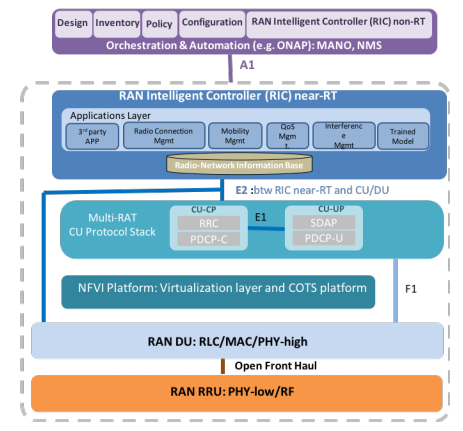
\includegraphics[width=0.8\textwidth]{./fig/oran1}
  \caption{ساختار شبکه ی \lr{ORAN} \cite{oranWP}}
  \label{fig:ORAN}
\end{figure}
اتحاد \lr{ORAN} در جستجوی چشم انداز باز بودن و هوشمندی برای شبکه های بی سیم نسل بعدی و فراتر از آن است.
\begin{itemize}
\item \textbf{باز بودن}:
ایجاد یک \lr{RAN} مقرون به صرفه نیاز به باز بودن ارتباط ها دارد.
رابط های باز برای فعال کردن فروشندگان و اپراتورهای کوچکتر به سرعت می توانند خدمات خود را معرفی کنند و یا اپراتورها را قادر می سازد تا شبکه را متناسب با نیازهای منحصر به فرد خود تنظیم کنند.
رابط های باز همچنین استقرار چند سازنده ای را قادر می سازد و اکوسیستم تأمین کننده رقابتی تر و پر جنب و جوش بیشتری را ایجاد می کند.
 همچنین نرم افزارهای منبع باز و طرحهای مرجع سخت افزار باعث نوآوری سریعتر و دموکراتیک تر می شود.
 \item \textbf{هوشمندی}
 شبکه ها با ظهور برنامه 5G پیچیده تر و متراکم تر شده و خواستار برنامه های غنی تر می شوند.
 برای کاستن این پیچیدگی نمی توان از ابزارهای سنتی انسانی  برای استقرار، بهینه سازی و بهره برداری از شبکه استفاده کرد.
 در نتیجه، شبکه ها باید خود متحرک شوندتا بتوانند از فن آوری های جدید مبتنی بر یادگیری برای خودکارسازی عملکرد شبکه های عملیاتی و کاهش \lr{OPEX} استفاده کنند.
 اتحاد \lr{ORAN} تلاش خواهد کرد تا از تکنیک های یادگیری عمیق در حال ظهور استفاده کند تا بتواند هر لایه از معماری \lr{RAN}  را به طور هوشمند پیاده سازی کند.
 پیاده سای هوشمند هم در مولفه ها و خم در سطح شبکه اعمال می گردد و منجر به تخصیص دینامیکی منابع رادیویی و بهینه سازی بازدهی شبکه می گردد.
 همراه با رابط های باز \lr{ORAN}، اتوماسیون حلقه بسته بهینه شده با هوش مصنوعی دست یافتنی است و دوره جدیدی را برای عملیات شبکه امکان پذیر می کند.
\end{itemize}

\lr{ORAN}، المانهای شبکه ی دسترسی رادیویی را مجازی می کند ، آنها را جدا کرده و رابط های باز مناسب را 
برای اتصال این عناصر
تعیین می کند. همچنین، 
\lr{ORAN}
از روشهای یادگیری ماشین برای هوشمندسازی لایه های 
\lr{RAN}
 استفاده می نماید. 
 در ساختار نوآورانه ی 
 \lr{ORAN}
 نرم افزار قابل برنامه ریزی 
 \lr{RAN}
 از سخت افزار جدا می شود.
  یکی از مهم ترین خصوصیات
  \lr{ORAN}
  رابط کاربری باز است که به اپراتورهای موبایل این قابلیت را می دهد تا بتوانند سرویس های مورد نیاز خود را تعریف نمایند.
  مفهوم 
  \lr{SDN}
  \LTRfootnote{software defined network}
  که مبنی بر جداسازی 
   بخش صفحه ی کنترل \lr{CP} از
   صفحه ی کاربر 
\lr{UP}
می باشد، در ساختار 
\lr{ORAN}
مورد بررسی قرار می گیرد.
این جداسازی منجر به بهبود 
\lr{RRM}
برای استفاده از زمان غیر واقعی و زمان نزدیک به واقعی در کنترلگر هوشمند شبکه ی دسترسی رادیویی \LTRfootnote{RAN Intelligent Controller} \lr{RIC} 
با استفاده از رابط های 
\lr{A1}
و
\lr{E2}
 می گردد.
همچنین 
منجر به جداسازی 
 \lr{CU}
 از 
 \lr{CP/UP}
 می شود
 که از طریق رابط \lr{E1} در 3GPP توسعه می یابد.

در ساختار
\lr{ORAN}،
واحد توزیع شده \lr{DU}،
نود منطقی می باشد که شامل لایه های 
\lr{RLC}
،
\lr{MAC}،
و
\lr{High-PHY}
است.
علاوه بر این، واحد مرکزی 
\lr{CU}
نود منطقی است که شامل لایه های 
\lr{RRC}،
\lr{SDAP} 
و 
\lr{PDCP}
می باشد.
نود منطقی واحد رادیویی
\lr{RU}
نیز، شامل لایه ی 
\lr{LOW-PHY}
و بخش پردازش رادیویی می باشد.
\lr{ORAN}
،
رابطهایی از جمله رابط 
\lr{fronthaul}
باز را شامل می شود که بخش \lr{DU} را به \lr{RU} متصل می نماید
(رابط 
\lr{E2}). 
همچنین
 رابط \lr{A1}
 بین لایه ی 
  \lr{orchestration/NMS}
  که شامل 
  تابع غیر واقعی زمان است و 
  \lr{eNB/qNB}
  که شامل تابع نزدیک به زمان است. 
\section{مجازی سازی توابع شبکه}
برای بهبود سرویس دهی در نسل پنجم مخابرات، جداسازی المان های نرم افزاری و سخت افزاری شبکه صورت گرفته است و به عنوان 
مجازی سازی توابع شبکه (\lr{NFV}) \LTRfootnote{network function virtualization}
معرفی شده است.
  حال توابع شبکه ی مجازی
  \lr{VNF}
  \LTRfootnote{Virtual network function} ،
  بلوکهای توابع سیستم هستند.
در نسل پنجم مخابرات 
  انتظار می رود که
   میزبان چندین سرویس
   با نیازهای مختلف به طور همزمان
    باشند.
 \section{برش شبکه}
 برش شبکه
 \LTRfootnote{Network Slicing}
به عنوان راه حلی برای چنین تقاضا در نظر گرفته شده است.
یک برش شبکه، یک شبکه منطقی \lr{end-to-end} است که خدمات  با نیازهای خاص را ارائه می دهد.
 چندین برش شبکه
در یک زیرساخت یکسان
  اجرا و مدیریت می شوند و
به طور مستقل کار کنید.
پیاده سازی های مختلفی از برش شبکه وجود دارد که شامل برش هسته ی شبکه، برش \lr{RAN} و برش هر دو بخش می باشد.
در برش هسته ی شبکه، برش تنها در بخش هسته ی شبکه است و تمام واسط ها و فرآیندها، بدون تغییر باقی می مانند.
در برش \lr{RAN}، 
برش های \lr{RAN}، بر روی   